\chapter{Methodology}\label{chap:Methodology}
To address the challenges identified in~\cref{chap:Related Work}, namely
evaluation-speed and categorization of near-classes, recent advances in machine
learning are considered. Contrary to most approaches in the field which perform
segmentation, our work focuses on detecting bounding boxes. In this chapter,
detail on the applied methods is provided. The methods are grouped as one-staged
or two-staged approaches. \todo{Shortly descripe what the difference between
one- and two-staged approaches is, what are the parts that are calculated 
(conf and loc)}

\section{Single Shot MultiBox Detector} Two common one-stage architectures are
\gls{yolo}~\cite{Redmon.20150608, Redmon.20161225, Redmon.20180409} and
\gls{ssd}~\cite{Liu.2016}. However, \gls{yolo} uses a singular base network
(Darknet \cite{JosephRedmon.20132016}). Therefore, \gls{ssd} was chosen over
\gls{yolo} for this paper, retaining the ability to quickly exchange base
networks.\\
This section describes central concepts of \gls{ssd}.

\subsection{SSD Architecture}\label{subsect:SSD Architecture}
As mentioned in the introduction to this section, \gls{ssd} is independent of a
specific base network. Exemplary, \autoref{fig:ssd-vgg} shows the architecure of
SSD for VGG16. Fully connected \glspl{layer} of VGG16 are dropped and replaced
with \glspl{convolutional layer}. We denote: 
\(Network:=Base\ Network\cup{}Additional\ Layers\).
Next, a set of \glspl{convolutional layer} \(L\subseteq Network\)
(blue and yellow in \autoref{fig:ssd-vgg}) \todo{maybe c=} is chosen from which
class- and bounding box predictions will be extracted. To simplify the task of
bounding box prediction, a set of \glspl{anchor} and a set of default boxes per
\gls{anchor} is computed as explained in
\autoref{subsect:Build up Default Boxes}. Now, instead of bounding boxes, offsets
to default boxes are predicted. This is done by running the individual
\gls{feature map} produced by every chosen \gls{layer} \(l\in L\) through a
subsequent \gls{convolutional layer} (green). The number of filters for the
subsequent \gls{layer} is chosen as \((4+c)*k\) with \(c\) classes and \(k\)
bounding boxes per \gls{anchor}. Therefore, the subsequent \gls{layer} of
\(l\in L\) with a \(m\times n\) \gls{feature map} produces \((4+c)kmn\) outputs.
A full prediction by \gls{ssd} returns the concatenation of outputs from all
chosen \glspl{layer}.

\todo{Note that each convolutional layer reduces the \gls{feature map} size. 
For computational details refer to \autoref{append:Convolutional Layer}}

\todo{Convolutional Layers, as thoroughly described in 
\autoref{append:Convolutional Layer} can be understood as a sliding window 
approach to neural networks.
In \gls{ssd}, each window is a prediction with an \gls{anchor} whereas 
\gls{yolo} uses a \gls{dense layer} instead.}
\begin{figure}[ht]
    \centering
    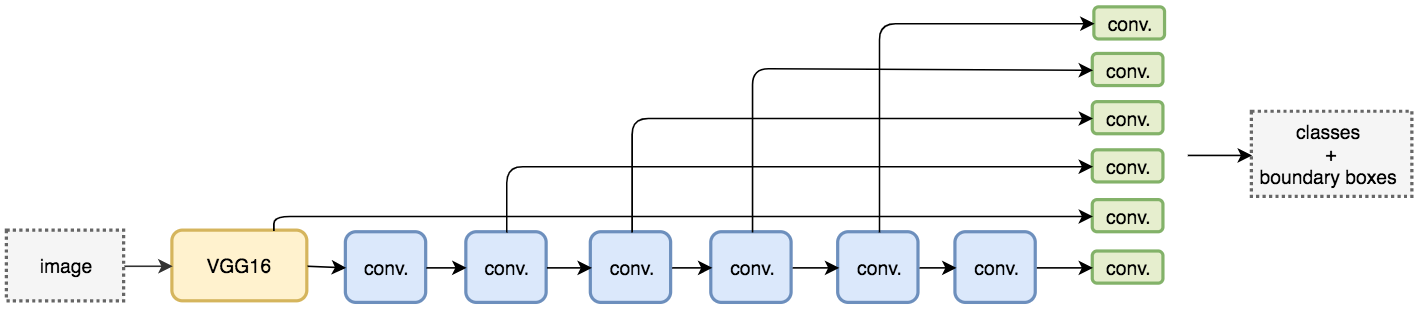
\includegraphics[width=1\textwidth]{vgg16-ssd}
    \caption{SSD upon VGG16}
    \label{fig:ssd-vgg}
\end{figure}\todo{cite}

\subsection{Build up Default Boxes}\label{subsect:Build up Default Boxes}
As described in \autoref{subsect:SSD Architecture}, a prediction is the output 
over all chosen \glspl{layer} \(L\subseteq Network\). Output of a \gls{layer} is 
a set of class predictions with respective default box offsets. However, 
convolutional \glspl{layer} in VGG16 decrease in size, either by pooling or 
stride. Therefore, a set of bounding boxes has to be computed for every chosen 
\gls{layer}.\\

\verysubsection{Anchor generation} \todo{Anchor does not use glossary here!}
As mentioned in \autoref{append:Convolutional Layer} the convolutional 
operation preserves spatial structure of a convolved image \(I\). To evenly 
tile the image with \glspl{anchor} in every \gls{layer} we make use of this property. 
Let \(I\) be an image of height \(h_I\) and width \(w_I\), let \(m\) be the 
\gls{feature map}, produced by a \gls{layer} \(l\in L\), with height \(h_m\) and
width \(w_m\). To relate \(I\) and \(m\), imagine upscaling \(m\). Then, 
the relative position of every original pixel in \(m\) is an \gls{anchor} in 
\(I\).\todo{This explanation is not exactly\dots cool.} The distance between
\glspl{anchor} is set by 
\begin{gather}
    dist_x=w_I/w_m\\
    dist_y=h_I/h_m
\end{gather}
We define the anchor \(a_i\), \(i\in [0, w_m*h_m]\) by its x- and y-coordinates 
\begin{gather}
    x_i=0.5*dist_x + \sum_{n=0}^{i-1} dist_x\\
    y_i=0.5*dist_y + \sum_{n=0}^{i-1} dist_y
\end{gather}
\autoref{fig:vgg16-anchors} shows results for an image \(I\) of height and width
\(I_w\times I_h=300\times 300\) and a \gls{feature map} \(m\) of height and
width \(m_w\times m_h=19\times 19\).
\begin{figure}[ht]
    \centering
    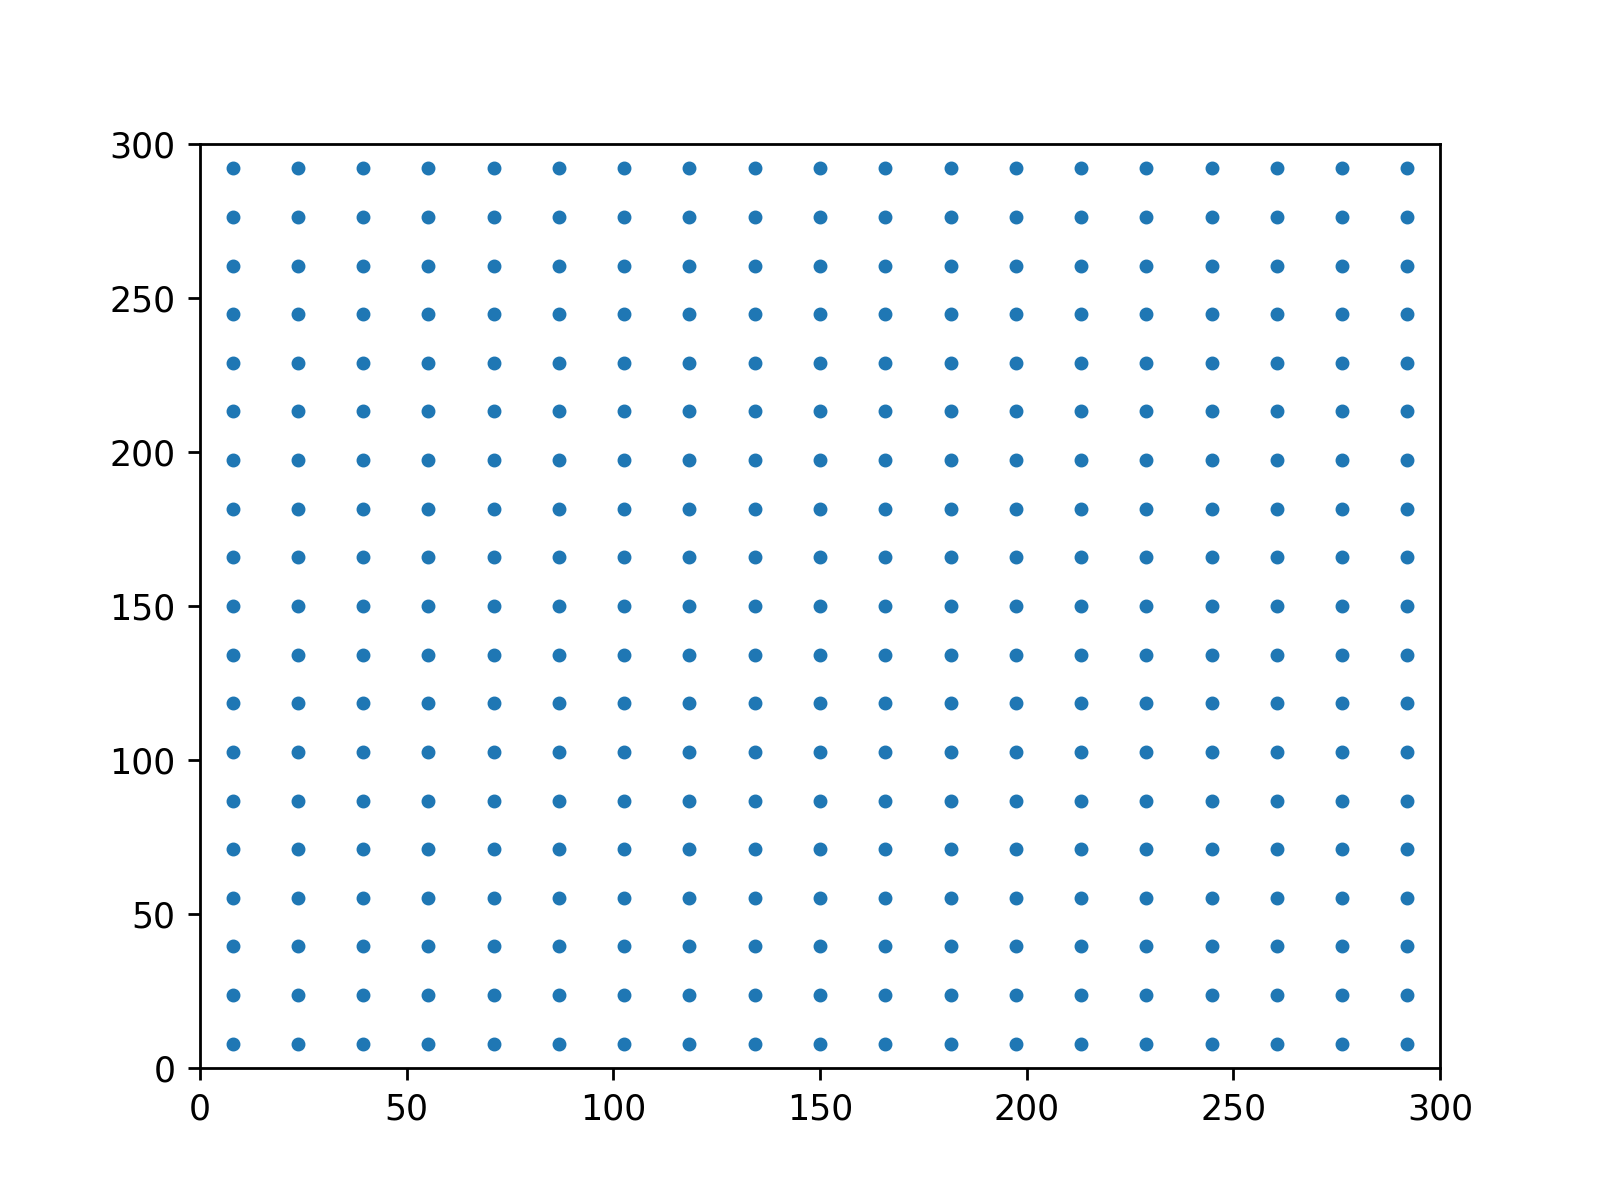
\includegraphics[width=0.5\textwidth]{vgg16-19x19}
    \caption{Generated anchors for an image (300x300) and \gls{feature map}(19x19))}
    \label{fig:vgg16-anchors}
\end{figure}\todo{cite}

\verysubsection{Default box size and aspect ratio}\label{verysubsect:Default box size and aspect ratio}
Suppose \(n=\abs{L}\). We calculate the size of default boxes for a feature map
\(m\) by \autoref{eq:default box size} as proposed in \cite{Liu.2016}
\begin{equation}
    s_m=s_{_\text{min}} + \frac{s_{_\text{max}}-s_{_\text{min}}}{n-1}(b-1)
\end{equation}\label{eq:default box size}
Where \(d\in [1, n]\), \(s_{_\text{min}}=0.2\) and \(s_{_\text{max}}=0.9\). To improve 
convergence, we find \(k\)-default box aspect ratios \(R\) by employing K-Means 
Clustering as described in \autoref{append:K-Means Clustering}, where \(k\) is 
dependent on the dataset.\todo{check whether is true later aswell.} We compute 
height and width of a default box with respect to an anchor \(a\in A_m\) (\(A_m\)
the set of all anchors for feature map \(m\)) as
\begin{equation}
    h_b^a=s_b\sqrt{a}\\
    w_b^a=s_b/\sqrt{a}
\end{equation}
Finally, the sets of default boxes per \gls{layer} are concatenated and further
encoded as described in \autoref{append:Concepts of Bounding Box Encoding}, such
that default box
\(\text{dbox} = \{\text{dbox}_{x_\text{min}}, \text{dbox}_{x_\text{max}}, \text{dbox}_{y_\text{min}}, \text{dbox}_{y_\text{max}}\}\)

\subsection{Encoding Ground Truth} For training, ground truth bounding boxes \(B\)
are encoded with respect to the concatenated default boxes as calculated in
\autoref{verysubsect:Default box size and aspect ratio}. \gls{ssd} is supposed
to infer offsets to default boxes (cf. \autoref{subsect:SSD Architecture}). To
simplify inference only default boxes with an intersect over union greater than
0.5 are chosen (cf. \autoref{sect:Intersect Over Union}). For a bounding box
\(\text{bbox}=\{\text{bbox}_{x_\text{min}}, \text{bbox}_{x_\text{max}}, \text{bbox}_{y_\text{min}}, \text{bbox}_{y_\text{max}}\}\), default box
\(\text{dbox}=\{\text{dbox}_{x_\text{min}}, \text{dbox}_{x_\text{max}}, \text{dbox}_{y_\text{min}}, \text{dbox}_{y_\text{max}}\}\) we compute the
encoded box \(\text{ebox}\) with \autoref{eq:encoded box}
\begin{equation}
    \text{ebox}=\{(\text{bbox}_{x_\text{min}}-\text{dbox}_{x_\text{min}}), (\text{bbox}_{x_\text{min}}-\text{dbox}_{x_\text{max}}), (\text{bbox}_{y_\text{min}}-\text{dbox}_{y_\text{max}})\}
\end{equation}\label{eq:encoded box}
We receive a matrix of dimensions \(\sum_{m\in M}{A_m}\times \sum_{m\in M}{k_m*4}\),
where \(M\) is the set fo all feature maps, \(A_m\) is the set of all anchors per
feature map and \(k_m\) is the amount of aspect ratios per feature map. Finally
we concatenate the class label to every encoded bounding box, such that the matrix
dimensions now are \(\sum_{m\in M}{A_m}\times \sum_{m\in M}{k_m*4+c}\), where c
is the amount of classes. Every row is now in the form of
\begin{equation}
    \left\{x_{_\text{min}}, x_{_\text{max}}, y_{_\text{min}}, y_{_\text{max}}, \text{one\_hot\_classes} \right\}
\end{equation}

\subsection{Train}
\blindtext[1]

\section{Faster R-CNN}
\blindtext[1]

\todo{Autoref does not work on equations - and verysubsect!!}